\documentclass[pdflatex,sn-aps]{sn-jnl}% American Physical Society (APS) Reference Style
%% iicol for multicols
%%%% My Packages
\usepackage{physics}
\usepackage{subcaption}
\usepackage{import}
\usepackage{xifthen}
\usepackage{pdfpages}
\usepackage{transparent}
\usepackage{physics}

\newcommand{\incfig}[1]{%
    \def\svgwidth{\columnwidth}
    \import{./figs/}{#1.pdf_tex}
}
%%%%

%%%% REMOVE BEFORE SUMBISSION
\usepackage{xcolor}
%%%%
\jyear{2022}%

\theoremstyle{thmstyleone}%
\newtheorem{theorem}{Theorem}%  meant for continuous numbers
\newtheorem{proposition}[theorem]{Proposition}% 

\theoremstyle{thmstyletwo}%
\newtheorem{example}{Example}%
\newtheorem{remark}{Remark}%

\theoremstyle{thmstylethree}%
\newtheorem{definition}{Definition}%

\raggedbottom%
%%\unnumbered% uncomment this for unnumbered level heads

\begin{document}

\title[Zonal Flow Persistent Homology]{Robust identification of Zonal Flow transitions using Persistent Homology}

%%=============================================================%%
%% Prefix	-> \pfx{Dr}
%% GivenName	-> \fnm{Joergen W.}
%% Particle	-> \spfx{van der} -> surname prefix
%% FamilyName	-> \sur{Ploeg}
%% Suffix	-> \sfx{IV}
%% NatureName	-> \tanm{Poet Laureate} -> Title after name
%% Degrees	-> \dgr{MSc, PhD}
%% \author*[1,2]{\pfx{Dr} \fnm{Joergen W.} \spfx{van der} \sur{Ploeg} \sfx{IV} \tanm{Poet Laureate} 
%%                 \dgr{MSc, PhD}}\email{iauthor@gmail.com}
%%=============================================================%%

\author*[1]{\fnm{Sage} \sur{Stanish}}\email{sagestanish@posteo.net}

\author[1]{\fnm{Sarah} \sur{Day}}\email{sldayx@wm.edu}
\equalcont{These authors contributed equally to this work.}

\author[2]{\fnm{Saskia} \sur{Mordijck}}\email{smordijck@wm.edu}
\equalcont{These authors contributed equally to this work.}

\author[3]{\fnm{Benjamin} \sur{Dudson}}\email{dudson2@llnl.gov}
\equalcont{These authors contributed equally to this work.}

\affil*[1]{\orgdiv{Department of Mathematics}, \orgname{College of William \& Mary}, \orgaddress{\street{Street}, \city{City}, \postcode{23187}, \state{VA}, \country{USA}}}

\affil[2]{\orgdiv{Department of Physics}, \orgname{College of William \& Mary}, \orgaddress{\street{Street}, \city{City}, \postcode{23187}, \state{VA}, \country{USA}}}

\affil[3]{\orgname{Lawrance Livermore National Laboratory}, \orgaddress{\city{Livermore}, \postcode{94550}, \state{CA}, \country{USA}}}

%%==================================%%
%% abstract %%
%%==================================%%

\abstract{}

\keywords{keyword1, Keyword2, Keyword3, Keyword4}

%%\pacs[JEL Classification]{D8, H51}

%%\pacs[MSC Classification]{35A01, 65L10, 65L12, 65L20, 65L70}

\maketitle

\section{Introduction}\label{sec:intro}

\par
Zonal Flows are a meso-scale turbulent flow observed in both fluid and plasma systems, such as the jet stream, ocean currents, Jovian atmospheres, and in magnetized plasmas~\cite{VASAVADA2005, VALLIS2017, DIAMOND2005}. In these systems, small scale turbulence self-organizes into flows which are characterized when using a Fourier decomposition with frequency, $\omega=0$ and wave number, $k=\infty$. They can be easily recognized on planets as large bands where fluids and plasmas flow and the beginning and tail of these flows connect.
\par
These flows are critical and act as a `transport barrier' to maintain a temperature gradient. Changes to these flows through changes in the free energy, typically through an increase in heating, that feeds the small scale turbulence drive can have detrimental impact. Climate change and a heating planet will impact atmospheric flows and ocean currents which will lead to changing local weather patterns~\cite{STENDEL2021}. In magnetized plasmas, zonal flows are instrumental in improving the confinement of the plasma by a factor 2, reducing the size of the fusion reactor~\cite{KEILHACKER1987}. The development of a robust mathematical technique, which does not rely on a human visual ad hoc assessment to identify the creation or disappearance of Zonal Flows.
\par
Topological Data Analysis is a emerging field in applied mathematics that offers techniques for studying topological features -- such as connected components and holes -- in image data.  It has proven useful in many scientific applications (\cite{} and references therein).  Particularly relevant is it's application to turbulence simulations\cite{} and verification of MHD models to experiment\cite{}.  We focus on the technique of persistent homology which extracts topological information from patterns in image data.  This technique benefits from a robustness against some forms of noise and is invariant under homeomorphic transformations of the image grid (re-scaling, stretching, etc).
%%% Should we add an image of DW versus ZF simulation from BOUT++? A:Sage: I think so, I will include the one from thesis.

In this paper, we show that the use of persistent homology allows us to computationally identify the transition from small scale turbulence to Zonal Flow regime using the Hasegawa-Wakatani model for plasma turbulence~\cite{HASEGAWA1983}. The Hasegawa-Wakatani model calculates drift-wave turbulence, which originates from a density gradient perpendicular to the magnetic field. The model is adapted by Numata et al.~\cite{NUMATA2007} to allow the generation of zonal-flows in a 2D system. These equations are solved numerically using the verified BOUT++ model~\cite{DUDSON2016}. In these simulations we can alter the free energy drive, by increasing the density gradient. $\kappa$, as well as the coupling parameters between the density and the potential fluctuations, referred to as the adiabacity, $\alpha$, which experimentally is often linked to the collisionality of the plasma.

The change from a pure drift-wave (DW) turbulence regime to a Zonal Flow (ZF) dominant regime is visually easy to identify through the appearance of large bands of uniform flows in the azymuthal direction. However, this change is not captured by Fourier decomposition and analysis requires a user to visually classify whether a transition has occurred, which leaves this open to human interpretation. Persistent homology mathematically analyzes the topology of the turbulence simulations by tracking the individual features and their topological lifespan. This new method of studying 2D visual turbulence provides the first method for identifying robustly different turbulence regimes and future work will expand this method to direct experimental observations.

\section{Results}\label{results}

Leveraging persistence homology analysis we can analyze a 2D-turbulence simulation using the Hasegawa-Wakatani model. As turbulence is characterized by a superposition of waves, the most common analysis technique to identify the turbulence characteristics relies on spectral analysis using a Fourier decomposition. Our results show that persistence homology can recreate the power spectrum characteristics, see section \ref{sec:fft}. Where spectral analysis fails at differentiation ZF from DW turbulence regimes, persistence homology analysis

    \subsection{Persistence}\label{res:persistence}
    \par
    Persistent homology (see \cite{computational_homology, tda_review}) is a mathematical construction from algebraic topology and in practice persistence diagrams -- summaries of persistent homology -- are used to analyse the information that persistent homology gives.  Persistence diagrams are a multi-set that contains the birth and death coordinates of each topological feature in a filtration of the target data.  In this work, we use a sublevel set filtration on 2D-greyscale images.  A sublevel set of an image $f:P\to U \subseteq \mathbb{R}$ for a set of pixels $P$ is
    \[f_t^- = \{p \in P \mid f(p) \leq t\}\]
    where $t\in U$ is called the filtration value.  Each of these sublevel sets is a binary image and the nested sequence, $\ldots \subset f_i^- \subset f_j^- \subset \ldots$ for all $i,j \in U$ such that $i<j$, is the sublevel set filtration of $f$.  Each sublevel has 2 associated topological features; $H_0$ features (connected components) and $H_1$ features (holes/enclosed regions).  The number of features in each sublevel changes as a function of filtration value.  The persistence diagram of $f$ is then the multi-set formed by triples $(n,b,d)$ where $b$ is the filtration value an $H_n$ feature first appears --- its birth --- and $d$ the value it disappears --- its death.  These diagrams are visually represented as a scatter plot with birth on the $x$-axis and death on the $y$-axis.  See fig \ref{fig:example_sublevel_sets} for an example of some sublevel sets, their associated number of features, and a full persistence diagram.  
\par
    Since our images are generated from a smooth, differenciable function (namely a well behaved simulation), the topological features are equivalent to a pairing of critical points.  $H_0$ features are born at local minima and die at local maxima/saddle points while $H_1$ features are born at minima/saddle points and die at local maxima\cite{tda_review, KP_morse}.  Intuitively, we then view each point on the persistence diagram as an individual pertebation in the image; $H_0$ feautres are negative `valleys' and $H_1$ features are positive `mountains'.  The lifespan --- defined as $l=b-d$ --- measures the intensity of the pertebation as the range between it's defining critical values.  Note that a features critical points need not be spacially local.  See figure \ref{fig:1d_per_ex} for a one dimensional example.  
    \begin{figure}[h]
        \centering
        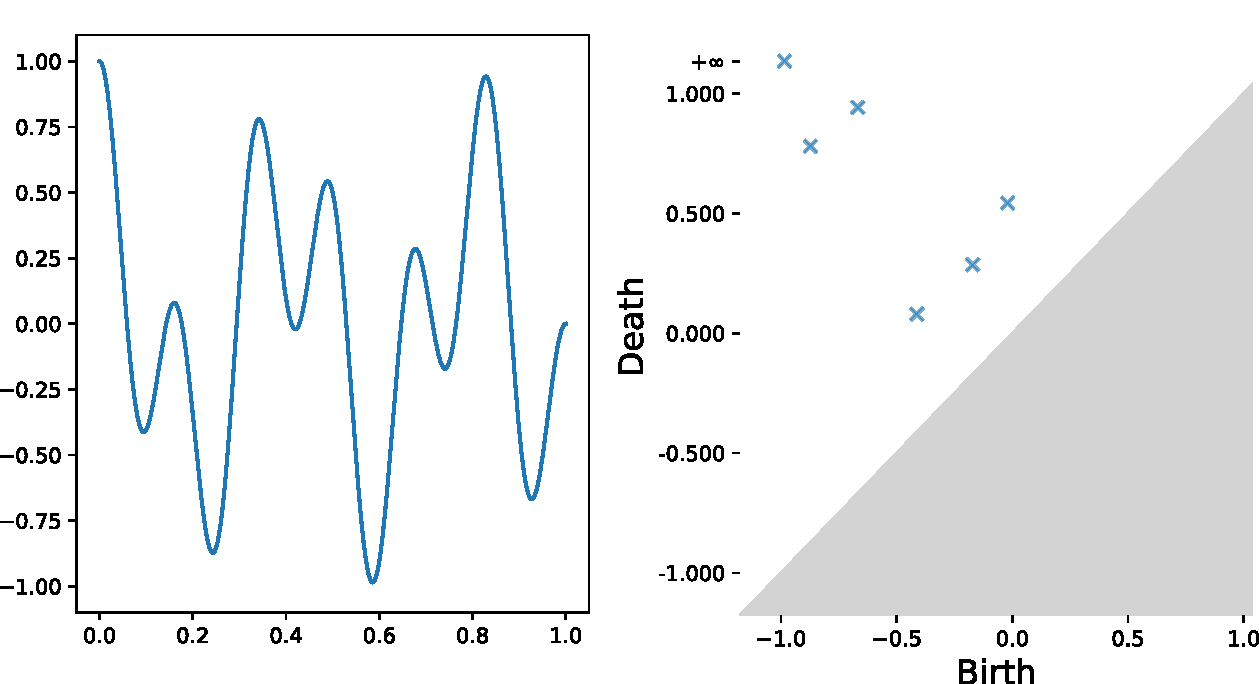
\includegraphics[width=\textwidth]{figs/1d_per_ex.png}%
        \caption[Example Persistence Diagram in One Dimension]{The persistent homology of a cosine wave (left) is represented in a persistence diagram (right).  The colored sections on the wave correspond to the colored points in the persistence diagram.  These features are a pairing of the colored critical points with a lifespan equal to the difference in their critical values (dotted line).  The three lower lifespan points in the diagram correspond to the three smaller perturbations in the data that rest on the three largest associated with the longer lifespan features. }%
        \label{fig:1d_per_ex}
    \end{figure}

\subsection{Identifying the Transition}\label{res:transition}

    \par
    We identify the DW-ZF transition in the MHW model as a change in the number of features in the persistent diagrams of density, $N_f(n(t,\alpha,\kappa))$.  In our simulations, the time averaged number of features, $\langle N_f(n) \rangle_t$ changes as a function of $\alpha$.  The $N_f$ curve --- fig (\ref{fig:number_of_features}) --- identifies three distinct regimes: turbulent $(\alpha < 0.0027)$, weakly zonal $( 0.0027 < \alpha < 0.027)$, and fully zonal $(0.027<\alpha)$.  
    \begin{figure}[h]
        \centering
        \textsc{Average Number of Features vs Kinetic/Zonal Energy Ration}
        \incfig{energy_vs_num_feat}
        %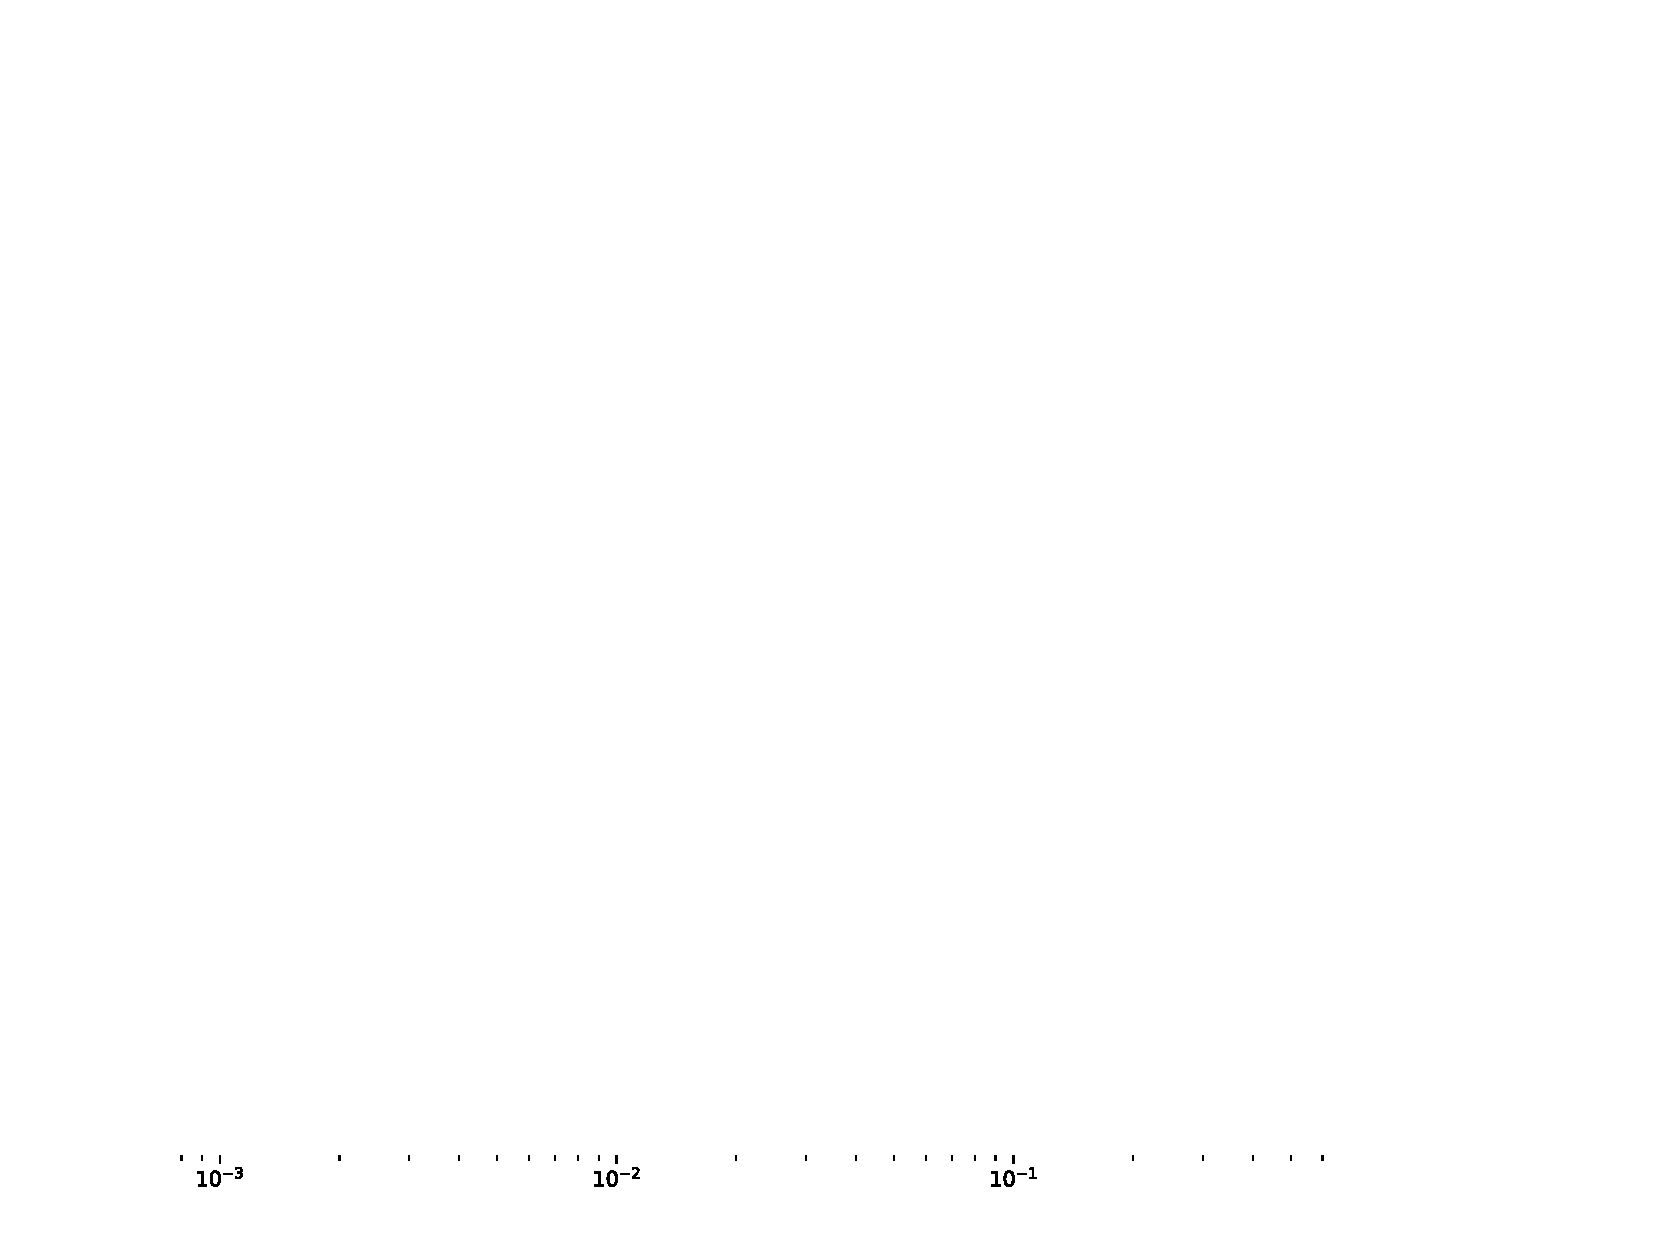
\includegraphics[width=\textwidth]{figs/energy_vs_num_feat.png}
        \caption{A plot of the number of features in persistent diagrams of $n$ over $\alpha$.  Overlayed on top of that is the ratio of zonal flow energy to total kinetic energy (red).  Each point in the graph is the average value of that metric over 200 independent images at that adiabaticity with error bars being one standard deviation.}\label{fig:number_of_features}
    \end{figure}

    \par
    The low $\alpha$ regime of the MHW model is known to be turbulent and increasing $\alpha$ drives more turbulence in the system.  $N_f$ picks up this increase in turbulence intensity as an increase in the number of features.  Stronger turbulence results in more waves of differing amplitude present in these images which implies a larger number of individual perturbations.  
    \par
    In the high $\alpha$ region, the MHW model is zonally dominated.  This is seen in example images of the density as large, flat regions of $0$ normalized density.  The zonal flows suppress nearly all the DW turbulence, so $N_f$ becomes small.  
    \par
    The in-between region --- $0.0027 < \alpha < 0.027$ --- has an exponentially decreasing $N_f$ as $\alpha \to 0.027$.  Images of the density in this region show the initial formation of zonal flows before they dominate the system.  These appear as horizontal striations where the DW turbulence is stretched in comparison the rest of the image.  The forming ZF's suppress some of the turbulence but are no strong enough to completely smooth out all the perturbations.  Persistence measures the exponential strengthening of ZF's as a decrease in the amount of turbulence.
    \par 
    This picture is slightly different from the more common technique used to identify the existence of ZF's.  Other literature has used a ratio of total kinetic energy --- $E_k =$ --- to Zonal Kinetic energy --- $E_z = $ --- to detect this transition.  The proper ratio for what is zonal or turbulent varies.  We follow the lead of Numata et. al\cite{NUMATA2007} and define $\frac{E_z}{E_k} < 20 \%$ as turbulent and $\frac{E_z}{E_k} > 80 \%$ as zonal.  
    \par
    This technique identifies a much broader transition region between Zonal and Turbulent states.  In particular, it fails to identify the weakly zonal regime that persistence does.  The turbulent regime ends as zonal flows begin to develop.  This is detected as an averaged movement of particles in the zonal direction.  Once there is some movement, the system is said zonal long before these flows become visible in still images of the density.  Zonal flows become fully developed once the amount of movement in the flow exceeds the defined threshold --- $80\%$ in this case.  This occurs before the DW turbulence is fully suppressed as can be seen in the images.  This is the key difference, the energy ration measures movement where-as persistence identifies differences in patterns.  
    \begin{figure}[h]
        \centering
        \incfig{regiemes}
        \caption{Example images of the MHW simulations at different $\alpha$.  Each image has its adiabacity printed below it.  The blue and red lines denote where persistence and the energy ratio partition parameter space.  Solid sections are Turbulent or Zonal and the dotted sections transitional.}
        \label{fig:regimes}
    \end{figure}

\subsection{Description of Transition}\label{res:description}

    \par
    Studying the persistent diagrams of these images gives insight into their structure.  Comparing these diagrams across the transition, we find \ldots (executive summery of section)

\subsubsection{Kolomogrov Scaling}

    \par
    Persistence reconstructs the Kolomogrov scaling in turbulent systems.  The lifespan of a feature measures the intensity of it's corresponding perturbation.  Since we are computing the persistence of a finite image, counting the number of features of a specific lifespan is a measure of density --- $\frac{N_f}{A}$.  Figure (\ref{fig:lifespan_vs_fourier}) shows the comparison of this lifespan data and the spacial Fourier power spectrum.  Both techniques clearly identify the exponential scaling of energy (amplitude/intensity) with spacial scale (frequency/density) that is indicative of turbulence.  
    \begin{figure}[h]
        \centering
        \textsc{Shape of Lifespan Distribution vs the Power Spectrum}\\
        \vspace{0.2cm}
        \begin{subfigure}{0.45\textwidth}
            \centering
            \incfig{lifespan_hist}
            \caption{\footnotesize Lifespan Histogram}\label{fig:lifespan_hist}
        \end{subfigure}
            \begin{subfigure}{0.45\textwidth}
            \centering
            \incfig{spectrum}
            \caption{\footnotesize Power Spectrum}\label{fig:power_spectra}
            \end{subfigure}
        \caption{Above is a comparison of persistence to the Fourier power spectrum.  Figure (a) is a normalized horizontal histogram of lifespan data.  Figure (b) plots the square norm of the $x$-directional Fourier transform vs frequency normalized across $z$.  Both figures are on a log-log scale.  Both techniques have a flat signal in the low frequency range before exponentially decreasing.  }%
        \label{fig:lifespan_comparison}
    \end{figure}


\subsubsection{Midlife}
\par
    Lifespan data decomposes a two dimensional persistent diagram into a one dimensional distribution.  A linearly independent measurement to lifespan is the feature midlife.  Midlife is defined as $\frac{\text{birth}+\text{death}}{2}$ and measures the vertical distance of a feature from the diagonal.  \ldots
    \par
    --- Need to pin down what we are saying with midlife.

\section{Discussion}

\section{Methods}\label{methods}
\par
Our data was generated using the example MHW model implemented in BOUT++ V4.4.  We fixed $\kappa=0.1$ and varied $\alpha$ logarithmicly through the transition region identified by Numata et al \cite{NUMATA2007}.  Each run is comprised of $30,000$ time steps where the rms of the density levels off after $10,000$.  Our data is a sample of every 100 time steps over the last $20,000$ --- the averaged autocorrelation of density becomes 0 at a spacing of 100 steps.  The simulation is then normalized along the $z$-axis to remove the background density gradient.  The persistent homology of each data point was computed using the gudhi python package v3.5.0 \cite{gudhi}.  
\backmatter%

\bmhead{Supplementary information}

\bmhead{Acknowledgments}

\section*{Declarations}

\begin{itemize}
\item Funding
\item Conflict of interest/Competing interests (check journal-specific guidelines for which heading to use)
\item Ethics approval 
\item Consent to participate
\item Consent for publication
\item Availability of data and materials
\par
Simulation data available at (Is there a better place to store?  I have half a terabyte of space at the following link and will upload the data there once I have internet speeds that will let me.): \url{www.filen.io}
\item Code availability 
\par
Code available at \url{https://github.com/sastanish/Robust-identification-of-Zonal-Flow-transitions-using-Persistent-Homology}
\item Authors' contributions
\end{itemize}

\begin{appendices}

\section{Section title of first appendix}\label{secA1}
%%=============================================%%
%% For submissions to Nature Portfolio Journals %%
%% please use the heading ``Extended Data''.   %%
%%=============================================%%
\end{appendices}

%%===========================================================================================%%
%% If you are submitting to one of the Nature Portfolio journals, using the eJP submission   %%
%% system, please include the references within the manuscript file itself. You may do this  %%
%% by copying the reference list from your .bbl file, paste it into the main manuscript .tex %%
%% file, and delete the associated \verb+\bibliography+ commands.                            %%
%%===========================================================================================%%

\bibliography{sn-bibliography}% common bib file
%% if required, the content of .bbl file can be included here once bbl is generated
%%\input sn-article.bbl

%% Default %%
%%\input sn-sample-bib.tex%

\end{document}
